Answering a question is a two-fold problem: The first part is actually understanding the question. A question is a query for a piece of knowledge, so the text of the question needs to be translated to a formal language. The second part is actually answering the question. Once the query is expressed in the right format, it needs to be executed on the knowledge base. Not every answer is stated explicitly in the knowledge base, so logical inference is required to combine multiple rules into a single answer. 
\subsection{Lexical analysis of questions}
The approach chosen by Krishnamurthy \cite{probseman} to parse the question is to actually reconstruct it from logical rules. The model is trained with manually translated questions. This allows the model to come up with possible rules and the likelihood that words and combinations of words translate into those rules. When the model is executed with a new question, it can look up the words and combine their corresponding rules from the bottom up. The probabilities calculated during training are used to decide at each step which of the options is the most likely.
\begin{figure}
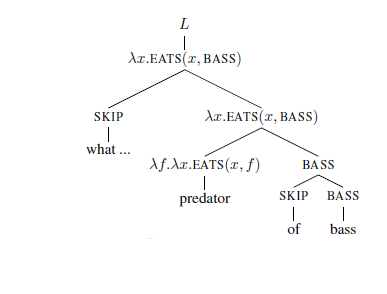
\includegraphics[width=0.48\textwidth]{parsetree}
\caption{The parse tree for the question ``What is the predator of bass?'' During training, the algorithm works from the top down to build the lexical rules. When the model is actually applied, these lexical rules are applied from the bottom up to come up with the final interpretation.}\label{fig:parsetree}
\end{figure}

\subsection{Querying the knowledge graph}
Once the meaning of the question is clear, an answer needs to be found in the knowledge base. The algorithm by Li and Clark \cite{sciencequestions} is one way to achieve that goal. After parsing the question, they extract keywords. Background knowledge is added, which results in a knowledge graph of concepts connected by the relations found in the knowledge base. These concepts are the keywords themselves, but also other related words which provide context. The questions are multiple choice, so each option is placed within that graph and connected to the other concepts. The answer that gets the highest confidence score in the knowledge graph is chosen as the solution.

\begin{figure}
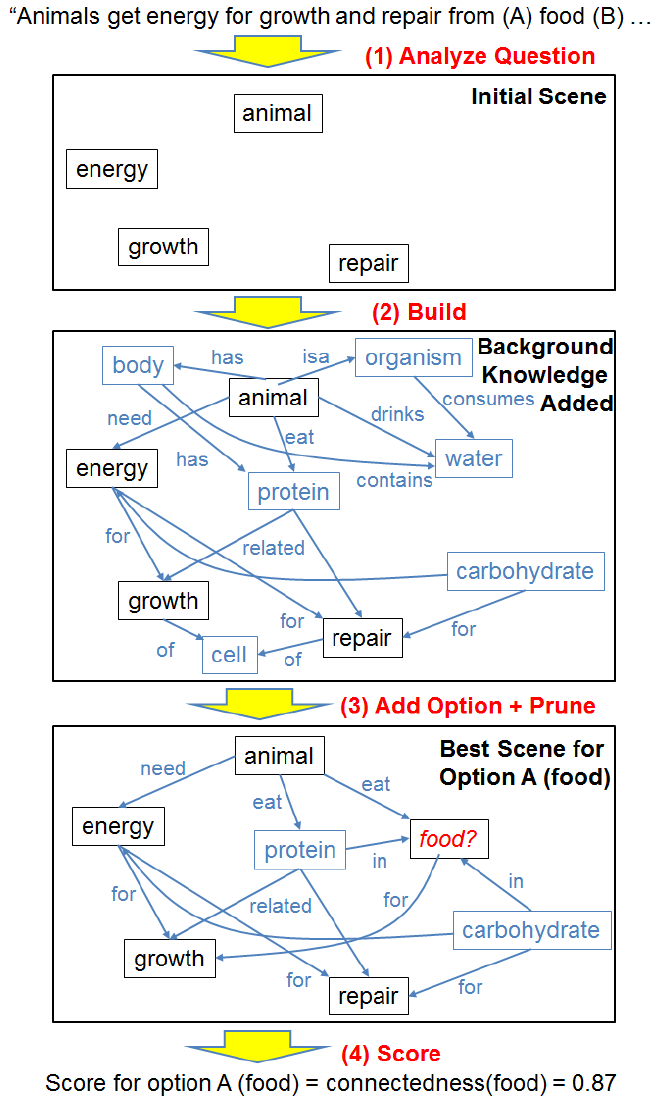
\includegraphics[width=0.48\textwidth]{graph}
\caption{An example of a question being answered using a knowledge graph.}\label{fig:parsetree}
\end{figure}